\chapter{Specifikacija programske potpore}
		
	\section{Funkcionalni zahtjevi}
			
			\noindent \textbf{Dionici:}
			
			\begin{packed_enum}
				
				\item Naručitelj
				\item Korisnici
				\begin{enumerate}
					\item Voditelj postaje
					\item Istraživač
					\item Tragač
				\end{enumerate}		
				\item Administrator
				\item Razvojni tim 
				
			\end{packed_enum}
			
			\noindent \textbf{Aktori i njihovi funkcionalni zahtjevi:}
			
			
			\begin{packed_enum}
				\item  \underbar{Neregistrirani korisnik (inicijator) može:}
				
				\begin{packed_enum}
					
					\item poslati zahtjev za registraciju s željenom ulogom za koju se prijavljuje
					
				\end{packed_enum}
				
			
				\item  \underbar{Voditelj postaje (inicijator) može:}
				
				\begin{packed_enum}
					
					\item dobiti pregled koji su tragači dio njegove postaje					
					\item dodati ili ukloniti tragače njegove postaje
					\item definirati na koji način su tragači osposobljeni izvoditi pretraživanje (pješke, dronom, automobilom, cross motorom, brodom ili helikopterom)
					\item odabrati konkretne tragače koji će sudjelovati u akciji
					\item ukloniti tragače s pojedine akcije po završetku njihova rada
					
				\end{packed_enum}
				
				\item  \underbar{Istraživač (inicijator) može:}
				
				\begin{packed_enum}
					
					\item dobiti pregled svih akcija koje je pokrenuo
					\item stvoriti nove akcije pretraživanja i praćenja s detaljima o određenim vrstama, jedinkama ili staništima za proučavanje
					\item poslati zahtjev za tragačima s opisom o potrebnim kvalifikacijama voditeljima postaja
					\item dobiti pregled koji tragači sudjeluju u akciji					
					\item preko karte tragačima pojedinačno zadati zadatke
					\item označiti da je neki tragač gotov sa svojim zadatkom
					\item ostaviti komentar za svaki zadatak
					\item bilježiti i vizualizirati staze kojima su tragači putovali i način kojim su se kretali u obliku toplinskih karata  
					\item odabrati da se za izradu interaktivnih karata koriste neka od idućih informacija: povijesne pozicije svih praćenih životinja, filtrirano po vrsti ili pojedinačno po jedinki te trenutne pozicije praćenih životinja 
					\item ostaviti komentar za ostale sudionike u akciji  
					
				\end{packed_enum}
				
				\item  \underbar{Tragač (inicijator) može:}
				
				\begin{packed_enum}
					 
					\item dobiti prikaz na karti zadataka koje treba obaviti, trenutne pozicije ostalih tragača aktivnih na istoj akciji, te trenutne pozicije praćenih životinja 
					\item ostaviti komentar za ostale sudionike u akciji
					\item ostaviti komentar praćenoj životinji tijekom akcije 
					
				\end{packed_enum}
				
				\item  \underbar{Administrator (inicijator) može:}
				
				\begin{packed_enum}
					
					\item potvrditi istraživača i voditelja postaje tijekom registracije
					\item vidjeti popis svih registriranih korisnika i njihovih osobnih podataka  
					\item mijenjati osobne podatke svih registriranih korisnika te njihove uloge
					
				\end{packed_enum}
				
				\item  \underbar{Baza podataka (sudionik):}
				
				\begin{packed_enum}
					
					\item pohranjuje sve podatke o korisnicima i njihovim ovlastima 
					\item pohranjuje sve podatke o akcijama, lokacijama, životinjama i sl. 
					
				\end{packed_enum}
			\end{packed_enum}
			
			\eject 
			
			
				
			\subsection{Obrasci uporabe}
								
					\noindent \underbar{\textbf{UC1 - Registracija}}
					\begin{packed_item}
	
						\item \textbf{Glavni sudionik:} Neregistrirani korisnik
						\item \textbf{Cilj:} Stvoriti korisnički račun za pristup sustavu
						\item \textbf{Sudionici:} Baza podataka
						\item \textbf{Preduvjet:} -
						\item \textbf{Opis osnovnog tijeka:}
						
						\item[] \begin{packed_enum}
	
							\item Korisnik odabire opciju za registraciju  
							\item Korisnik unosi potrebne korisničke podatke (korisničko ime, fotografija, lozinka, ime, prezime i email adresa) te odabire željenu ulogu za koju se prijavljuje 
							\item Korisnik prima obavijest o uspješnoj/neuspješnoj registraciji
						\end{packed_enum}
						
						\item  \textbf{Opis mogućih odstupanja:}
						
						\item[] \begin{packed_item}
	
							\item[2.a] Odabir već zauzetog korisničkog imena i/ili e-maila, unos korisničkog podatka u nedozvoljenom formatu ili pružanje neispravnoga e-maila 
							\item[] \begin{packed_enum}
								
								\item Sustav obavještava korisnika o neuspjelom upisu i vraća ga na stranicu za registraciju 
								\item Korisnik mijenja potrebne podatke te završava unos ili odustaje od registracije 
								
							\end{packed_enum}
							\item[3.a] Administrator odbija registraciju korisnika koji se želi registrirati kao istraživač ili voditelj postaje
							\item[] \begin{packed_enum}
								
								\item Sustav obavještava korisnika o neuspjelom upisu i vraća ga na stranicu za registraciju 
								
							\end{packed_enum}
							
						\end{packed_item}
					\end{packed_item}
				
					\noindent \underbar{\textbf{UC2 - Prijava u sustav}}
					\begin{packed_item}
						
						\item \textbf{Glavni sudionik:} Korisnik
						\item \textbf{Cilj:} Dobiti pristup korisničkom sučelju 
						\item \textbf{Sudionici:} Baza podataka 
						\item \textbf{Preduvjet:} Korisnik ima registrirani korisnički račun
						\item \textbf{Opis osnovnog tijeka:}
						
						\item[] \begin{packed_enum}
							
							\item Unos korisničkog imena i lozinke 
							\item Potvrda o ispravnosti unesenih podataka 
							\item Pristup korisničkim funkcijama
						\end{packed_enum}
						
						\item  \textbf{Opis mogućih odstupanja:}
						
						\item[] \begin{packed_item}
							
							\item[2.a] Neispravno korisničko ime/lozinka
							\item[] \begin{packed_enum}
								
								\item Sustav obavještava korisnika o neuspjelom upisu i vraća ga na stranicu za registraciju
								
							\end{packed_enum}
							
						\end{packed_item}
					\end{packed_item}
					
					\noindent \underbar{\textbf{UC3 - Pregled osobnih podataka}}
					\begin{packed_item}
						
						\item \textbf{Glavni sudionik:} Korisnik
						\item \textbf{Cilj:} Pregledati osobne podatke
						\item \textbf{Sudionici:} Baza podataka
						\item \textbf{Preduvjet:} Korisnik je prijavljen
						\item \textbf{Opis osnovnog tijeka:}
						
						\item[] \begin{packed_enum}
							
							\item Korisnik odabire opciju ”Osobni podatci” 
							\item Sustav prikazuje osobne podatke korisnika
						\end{packed_enum}
					\end{packed_item}
					
					\noindent \underbar{\textbf{UC4 - Pregled članova postaje}}
					\begin{packed_item}
						
						\item \textbf{Glavni sudionik:} Voditelj postaje
						\item \textbf{Cilj:} Dobiti popis tragača koji su članovi postaje
						\item \textbf{Sudionici:} Baza podataka
						\item \textbf{Preduvjet:} Voditelj postaje je prijavljen
						\item \textbf{Opis osnovnog tijeka:}
						
						\item[] \begin{packed_enum}
							
							\item Voditelj bira opciju "Članovi postaje" 
							\item Sustav prikazuje popis tragača koji su članovi postaje
						\end{packed_enum}
					\end{packed_item}
					
					\noindent \underbar{\textbf{UC5 - Dodavanje tragača u postaju}}
					\begin{packed_item}
						
						\item \textbf{Glavni sudionik:} Voditelj postaje
						\item \textbf{Cilj:} Dodati slobodnog tragača među članove postaje
						\item \textbf{Sudionici:} Baza podataka, tragač
						\item \textbf{Preduvjet:} Voditelj postaje je prijavljen
						\item \textbf{Opis osnovnog tijeka:}
						
						\item[] \begin{packed_enum}
							
							\item Voditelj postaje bira opciju "Dodaj tragača u postaju" 
							\item Sustav prikazuje popis slobodnih tragača
							\item Voditelj odabire tragače koje želi dodijeliti svojoj postaji 
							\item Voditelj potvrđuje odabir 
							\item Sustav ažurira bazu podataka i dodjeljuje odabrane tragače postaji koju vodi voditelj
						\end{packed_enum}
						
						\item  \textbf{Opis mogućih odstupanja:}
						
						\item[] \begin{packed_item}
							
							\item[1.a] Ne postoji registrirani tragač koji već nije član neke postaje
							\item[] \begin{packed_enum}
								
								\item Sustav obavještava korisnika o nepostojanju slobodnih tragača
								
							\end{packed_enum}
							
						\end{packed_item}
					\end{packed_item}
					
					\eject
					
					\noindent \underbar{\textbf{UC6 - Uklanjanje tragača iz postaje}}
					\begin{packed_item}
						
						\item \textbf{Glavni sudionik:} Voditelj postaje
						\item \textbf{Cilj:} Ukloniti tragača iz članova postaje
						\item \textbf{Sudionici:} Baza podataka, tragač
						\item \textbf{Preduvjet:} Voditelj postaje je prijavljen i postoje tragači koji pripadaju njegovoj postaji
						\item \textbf{Opis osnovnog tijeka:}
						
						\item[] \begin{packed_enum}
							
							\item Voditelj postaje bira opciju "Ukloni tragača iz postaje" 
							\item Sustav prikazuje popis tragača koji su članovi postaje
							\item Voditelj odabire tragače koje želi ukloniti iz svoje postaje 
							\item Voditelj potvrđuje odabir 
							\item Sustav ažurira bazu podataka i odabrane tragače dodaje na listu slobodnih tragača
						\end{packed_enum}
					\end{packed_item}
					
					\noindent \underbar{\textbf{UC7 - Definiranje osposobljenosti tragača}}
					\begin{packed_item}
						
						\item \textbf{Glavni sudionik:} Voditelj postaje
						\item \textbf{Cilj:} Definirati na koji način su tragači osposobljeni izvoditi pretraživanje (pješke, dronom, automobilom, cross motorom, brodom ili helikopterom)
						\item \textbf{Sudionici:} Baza podataka, tragač
						\item \textbf{Preduvjet:} Voditelj je prijavljen i postoje tragači koji pripadaju njegovoj postaji
						\item \textbf{Opis osnovnog tijeka:}
						
						\item[] \begin{packed_enum}
							
							\item Sustav prikazuje popis tragača koji su članovi postaje
							\item Voditelj postaje odabire tragača 
							\item Voditelj odabire opciju "Definiraj osposobljenost tragača" 
							\item Voditelj odabire koja osposobljenja za način pretraživanja ima tragač
							\item Voditelj potvrđuje odabir 
							\item Sustav ažurira bazu podataka s odabranim načinima pretraživanja
						\end{packed_enum}
					\end{packed_item}
					
					\noindent \underbar{\textbf{UC8 - Pregled zahtjeva za tragačima}}
					\begin{packed_item}
						
						\item \textbf{Glavni sudionik:} Voditelj postaje
						\item \textbf{Cilj:} Dobiti popis pristiglih zahtjeva za alociranje tragača za sudjelovanje u akciji
						\item \textbf{Sudionici:} Baza podataka
						\item \textbf{Preduvjet:} Voditelj je prijavljen
						\item \textbf{Opis osnovnog tijeka:}
						
						\item[] \begin{packed_enum}
							
							\item Voditelj odabire opciju "Pristigli zahtjevi"
							\item Sustav prikazuje popis pristiglih zahtjeva za alociranje tragača za sudjelovanje u akciji
						\end{packed_enum}
					\end{packed_item}
					
					
					\noindent \underbar{\textbf{UC9 - Odabir tragača za akciju}}
					\begin{packed_item}
						
						\item \textbf{Glavni sudionik:} Voditelj postaje
						\item \textbf{Cilj:} Odabrati koji tragači će sudjelovati u nekoj akciji
						\item \textbf{Sudionici:} Baza podataka, tragač
						\item \textbf{Preduvjet:} Voditelj je prijavljen i primio je barem jedan zahtjev za alociranjem tragača za sudjelovanje u akciji
						\item \textbf{Opis osnovnog tijeka:}
						
						\item[] \begin{packed_enum}
							
							\item Sustav prikazuje zahtjev za alociranjem tragača za sudjelovanje u akciji
							\item Voditelj postaje odabire opciju "Odaberi tragače za akciju"
							\item Sustav prikazuje popis raspoloživih tragača
							\item Voditelj odabire tragača
							\item Voditelj potvrđuje odabir
							\item Sustav ažurira bazu podataka i dodjeljuje odabrane tragače akciji 
						\end{packed_enum}
						
						\item  \textbf{Opis mogućih odstupanja:}
						
						\item[] \begin{packed_item}
							
							\item[2.a] Nema raspoloživih tragača
							\item[] \begin{packed_enum}
								
								\item Sustav obavještava voditelj o nedostatku raspoloživih tragača								
							\end{packed_enum}
							
						\end{packed_item}
						
					\end{packed_item}
					
					\noindent \underbar{\textbf{UC10 - Uklanjanje tragača s akcije}}
					\begin{packed_item}
						
						\item \textbf{Glavni sudionik:} Voditelj postaje
						\item \textbf{Cilj:} Odabrati koji tragači će sudjelovati u nekoj akciji
						\item \textbf{Sudionici:} Baza podataka, tragač
						\item \textbf{Preduvjet:} Voditelj je prijavljen i tragač sudjeluje u nekoj akciji
						\item \textbf{Opis osnovnog tijeka:}
						
						\item[] \begin{packed_enum}
							
							\item Sustav prikazuje popis tragača koji su članovi postaje 
							\item Voditelj odabire tragača kojeg želi ukloniti s neke akcije
							\item Voditelj odabire opciju "Ukloni s akcije"
							\item Voditelj potvrđuje odabir
							\item Sustav ažurira bazu podataka i vraća tragača na popis raspoloživih tragača
						\end{packed_enum}
						
						\item  \textbf{Opis mogućih odstupanja:}
						
						\item[] \begin{packed_item}
							
							\item[3.a] Tragač nije završio sa zadatkom na akciji
							\item[] \begin{packed_enum}
								
								\item Sustav obavještava voditelja da mu nije dopušteno ukloniti tragača s akcije			
							\end{packed_enum}
							
						\end{packed_item}
						
					\end{packed_item}
					
					\noindent \underbar{\textbf{UC11 - Pregled akcija}}
					\begin{packed_item}
						
						\item \textbf{Glavni sudionik:} Istraživač
						\item \textbf{Cilj:} Dobiti popis akcija u kojima istraživač sudjeluje
						\item \textbf{Sudionici:} Baza podataka
						\item \textbf{Preduvjet:} Istraživač je prijavljen
						\item \textbf{Opis osnovnog tijeka:}
						
						\item[] \begin{packed_enum}
							
							\item Istraživač odabire opciju "Moje akcije" 
							\item Sustav prikazuje popis akcija u kojima istraživač sudjeluje
						\end{packed_enum}
					\end{packed_item}
					
					\noindent \underbar{\textbf{UC12 - Stvaranje novih akcija}}
					\begin{packed_item}
						
						\item \textbf{Glavni sudionik:} Istraživač
						\item \textbf{Cilj:} Stvoriti novu akciju pretraživanja i praćenja s detaljima o određenim vrstama, jedinkama ili staništima za proučavanje
						\item \textbf{Sudionici:} Baza podataka
						\item \textbf{Preduvjet:} Istraživač je prijavljen
						\item \textbf{Opis osnovnog tijeka:}
						
						\item[] \begin{packed_enum}
							
							\item Istraživač odabire opciju "Stvori novu akciju" 
							\item Sustav prikazuje obrazac za unos detalja o akciji 
							\item Istraživač unosi tražene podatke 
							\item Istraživač potvrđuje unos 
							\item Sustav ažurira bazu podataka s novom akcijom 
						\end{packed_enum}
					\end{packed_item}
					
					\noindent \underbar{\textbf{UC13 - Slanje zahtjeva za tragačima}}
					\begin{packed_item}
						
						\item \textbf{Glavni sudionik:} Istraživač
						\item \textbf{Cilj:} Poslati zahtjev za tragačima s opisom o potrebnim kvalifikacijama voditeljima postaja
						\item \textbf{Sudionici:} Baza podataka, voditelj postaje
						\item \textbf{Preduvjet:} Istraživač je prijavljen i postoji barem jedan voditelj postaje s tragačima u svojoj postaji
						\item \textbf{Opis osnovnog tijeka:}
						
						\item[] \begin{packed_enum}
							
							\item Istraživač odabire opciju "Pošalji zahtjev za tragačima" 
							\item Sustav prikazuje obrazac za unos detalja o zahtjevu (kvalifikacije, broj tragača, itd.) 
							\item Istraživač unosi tražene podatke 
							\item Istraživač odabire postaju kojoj želi poslati zahtjev
							\item Istraživač potvrđuje slanje zahtjeva
							\item Sustav ažurira bazu podataka s poslanim zahtjevom
						\end{packed_enum}
					\end{packed_item}
					
					\noindent \underbar{\textbf{UC14 - Pregled članova akcije}}
					\begin{packed_item}
						
						\item \textbf{Glavni sudionik:} Istraživač
						\item \textbf{Cilj:} Dobiti popis tragača koji sudjeluju u akciji
						\item \textbf{Sudionici:} Baza podataka
						\item \textbf{Preduvjet:} Istraživač je prijavljen
						\item \textbf{Opis osnovnog tijeka:}
						
						\item[] \begin{packed_enum}
							
							\item Sustav prikazuje popis akcija u kojima istraživač sudjeluje
							\item Istraživač odabire akciju
							\item Istraživač odabire opciju "Članovi akcije"
							\item Sustav prikazuje popis tragača koji sudjeluju u akciji
						\end{packed_enum}
					\end{packed_item}
					
					\noindent \underbar{\textbf{UC15 - Dodjela zadatka tragaču}}
					\begin{packed_item}
						
						\item \textbf{Glavni sudionik:} Istraživač
						\item \textbf{Cilj:} Dodijeliti određen zadatak akcije nekom tragaču koji sudjeluje u akciji
						\item \textbf{Sudionici:} Baza podataka, tragač
						\item \textbf{Preduvjet:} Istraživač je prijavljen i postoji barem jedan tragač koji sudjeluje u akciji
						\item \textbf{Opis osnovnog tijeka:}
						
						\item[] \begin{packed_enum}
							
							\item Sustav prikazuje popis tragača koji sudjeluju u akciji
							\item Istraživač odabire tragača kojem želi dodijeliti zadatak
							\item Istraživač odabire opciju "Dodijeli zadatak tragaču" 
							\item Sustav prikazuje kartu
							\item Istraživač odabire rutu i odredišnu lokaciju zadatka
							\item Istraživač odabire koji uređaj želi da bude postavljen(kamera ili uređaj za praćenje) 
							\item Istraživač potvrđuje dodjelu zadatka 
							\item Sustav ažurira bazu podataka s dodijeljenim zadatkom tragaču 				
						\end{packed_enum}
					\end{packed_item}
					
					\noindent \underbar{\textbf{UC16 - Pregled zadataka}}
					\begin{packed_item}
						
						\item \textbf{Glavni sudionik:} Istraživač
						\item \textbf{Cilj:} Dobiti popis zadataka zadanih u akciji
						\item \textbf{Sudionici:} Baza podataka
						\item \textbf{Preduvjet:} Istraživač je prijavljen
						\item \textbf{Opis osnovnog tijeka:}
						
						\item[] \begin{packed_enum}
							
							\item Sustav prikazuje popis akcija u kojima istraživač sudjeluje
							\item Istraživač odabire akciju
							\item Istraživač odabire opciju "Pregled zadataka"
							\item Sustav prikazuje popis zadataka koje je istraživač dodijelio
						\end{packed_enum}
					\end{packed_item}
					
					\noindent \underbar{\textbf{UC17 - Ostavljanje komentara za zadatak}}
					\begin{packed_item}
						
						\item \textbf{Glavni sudionik:} Istraživač
						\item \textbf{Cilj:} Ostaviti komentar za neki zadatak
						\item \textbf{Sudionici:} Baza podataka
						\item \textbf{Preduvjet:} Istraživač je prijavljen i dodijelio je barem jedan zadatak
						\item \textbf{Opis osnovnog tijeka:}
						
						\item[] \begin{packed_enum}
							
							\item Sustav prikazuje popis zadataka koje je istraživač dodijelio
							\item Istraživač odabire zadatak
							\item Istraživač odabire opciju "Ostavi komentar" 
							\item Istraživač unosi željeni komentar 
							\item Istraživač potvrđuje unos 
							\item Sustav ažurira bazu podataka s novim komentarom za zadatak 
						\end{packed_enum}
					\end{packed_item}
					
					\noindent \underbar{\textbf{UC18 - Proglašenje zadatka dovršenim}}
					\begin{packed_item}
						
						\item \textbf{Glavni sudionik:} Istraživač
						\item \textbf{Cilj:} Označiti da je neki zadatak dovršen
						\item \textbf{Sudionici:} Baza podataka
						\item \textbf{Preduvjet:} Istraživač je prijavljen i dodijelio je barem jedan zadatak
						\item \textbf{Opis osnovnog tijeka:}
						
						\item[] \begin{packed_enum}
							
							\item Sustav prikazuje popis zadataka koje je istraživač dodijelio
							\item Istraživač odabire zadatak
							\item Istraživač odabire opciju "Označi dovršenim" 
							\item Istraživač potvrđuje unos 
							\item Sustav ažurira bazu podataka s oznakom da je tragač završio zadatak 
						\end{packed_enum}
					\end{packed_item}
					
					\noindent \underbar{\textbf{UC19 - Prikaz interaktivne karte}}
					\begin{packed_item}
						
						\item \textbf{Glavni sudionik:} Istraživač
						\item \textbf{Cilj:} Stvoriti interaktivnu kartu
						\item \textbf{Sudionici:} Baza podataka
						\item \textbf{Preduvjet:} Istraživač je prijavljen
						\item \textbf{Opis osnovnog tijeka:}
						
						\item[] \begin{packed_enum}
							
							\item Istraživač odabire opciju "Karta" 
							\item Sustav učitava kartu s posljednjim spremljenim promjenama
						\end{packed_enum}
					\end{packed_item}
					
					\noindent \underbar{\textbf{UC20 - Uređivanje interaktivne karte}}
					\begin{packed_item}
						
						\item \textbf{Glavni sudionik:} Istraživač
						\item \textbf{Cilj:} Stvoriti interaktivnu kartu
						\item \textbf{Sudionici:} Baza podataka
						\item \textbf{Preduvjet:} Istraživač je prijavljen
						\item \textbf{Opis osnovnog tijeka:}
						
						\item[] \begin{packed_enum}
							
							\item Istraživač odabire opciju "Uredi kartu"
							\item Sustav prikazuje opcije informacija koje mogu biti prikazane na karti
							\item Istraživač uređuje kartu prema svojim potrebama
							\item Istraživač potvrđuje promjene
							\item Sustav pohranjuje interaktivnu kartu u bazu podataka 
						\end{packed_enum}
					\end{packed_item}
					
					\noindent \underbar{\textbf{UC21 - Ostavljanje komentara na karti}}
					\begin{packed_item}
						
						\item \textbf{Glavni sudionik:} Istraživač, tragač
						\item \textbf{Cilj:} Ostaviti komentar na karti drugim sudionicima akcije
						\item \textbf{Sudionici:} Baza podataka
						\item \textbf{Preduvjet:} Istraživač ili tragač je prijavljen i sudjeluje u akciji
						\item \textbf{Opis osnovnog tijeka:}
						
						\item[] \begin{packed_enum}
							
							\item Sustav prikazuje kartu
							\item Istraživač ili tragač odabire opciju "Ostavi komentar" 
							\item Istraživač ili tragač unosi željeni komentar 
							\item Istraživač ili tragač potvrđuje unos 
							\item Sustav ažurira bazu podataka s novim komentarom za sudionike akcije 
						\end{packed_enum}
					\end{packed_item}
					
					\noindent \underbar{\textbf{UC22 - Ostavljanje komentara za praćenu životinju}}
					\begin{packed_item}
						
						\item \textbf{Glavni sudionik:} Tragač
						\item \textbf{Cilj:} Ostaviti komentar praćenoj životinji 
						\item \textbf{Sudionici:} Baza podataka
						\item \textbf{Preduvjet:} Tragač je prijavljen i sudjeluje u akciji
						\item \textbf{Opis osnovnog tijeka:}
						
						\item[] \begin{packed_enum}
							
							\item Tragač odabire opciju "Ostavi komentar za životinju" 
							\item Sustav prikazuje polje za unos komentara 
							\item Tragač unosi željeni komentar 
							\item Tragač potvrđuje unos 
							\item Sustav ažurira bazu podataka s novim komentarom za praćenu životinju 
						\end{packed_enum}
					\end{packed_item}
					
					\noindent \underbar{\textbf{UC23 - Pregled karte}}
					\begin{packed_item}
						
						\item \textbf{Glavni sudionik:} Tragač
						\item \textbf{Cilj:} Pristupiti karti za pregled zadataka koje treba obaviti, trenutne pozicije ostalih tragača aktivnih na istoj akciji, te trenutne pozicije praćenih životinja
						\item \textbf{Sudionici:} Baza podataka
						\item \textbf{Preduvjet:} Tragač je prijavljen i sudjeluje u akciji 
						\item \textbf{Opis osnovnog tijeka:}
						
						\item[] \begin{packed_enum}
							
							\item Tragač odabire opciju "Karta" 
							\item Sustav prikazuje kartu s označenim zadacima, pozicijama tragača i praćenih životinja 
							\item Tragač može interaktivno pregledavati kartu i pratiti informacije o akciji
						\end{packed_enum}
					\end{packed_item}
					
					\noindent \underbar{\textbf{UC24 - Pregled zahtjeva za registracijom}}
					\begin{packed_item}
						
						\item \textbf{Glavni sudionik:} Administrator
						\item \textbf{Cilj:} Dobiti popis svih pristiglih zahtjeva za registracijom u ulozi voditelja postaje ili istraživača
						\item \textbf{Sudionici:} Baza podataka
						\item \textbf{Preduvjet:} Korisnik je registriran i dodijeljena su mu prava administratora te postoji barem jedan zahtjev za registracijom u ulozi voditelja ili istraživača
						\item \textbf{Opis osnovnog tijeka:}
						
						\item[] \begin{packed_enum}
							
							\item Administrator odabire opciju "Pristigli zahtjevi"
							\item Sustav prikazuje popis pristiglih zahtjeva za registraciju u u ulozi voditelja postaje ili istraživača 
						\end{packed_enum}
					\end{packed_item}
					
					\noindent \underbar{\textbf{UC25 - Potvrda registracije}}
					\begin{packed_item}
						
						\item \textbf{Glavni sudionik:} Administrator
						\item \textbf{Cilj:} Potvrditi/odbiti registraciju korisnika koji se želi registrirati kao istraživač ili voditelj postaje
						\item \textbf{Sudionici:} Baza podataka, neregistrirani korisnik
						\item \textbf{Preduvjet:} Korisnik je registriran i dodijeljena su mu prava administratora
						\item \textbf{Opis osnovnog tijeka:}
						
						\item[] \begin{packed_enum}
							
							\item Sustav prikazuje popis pristiglih zahtjeva za registraciju u ulozi voditelja postaje ili istraživača
							\item Administrator odabire zahtjev 
							\item Administrator odabire opciju "Potvrdi" ili "Odbij"
							\item Ako administrator odabere opciju potvrdi, sustav ažurira bazu podataka s novim korisnikom
						\end{packed_enum}
					\end{packed_item}
					
					\noindent \underbar{\textbf{UC26 - Pregled svih korisnika}}
					\begin{packed_item}
						
						\item \textbf{Glavni sudionik:} Administrator
						\item \textbf{Cilj:} Pregledati sve registrirane korisnike i njihove osobne podatke
						\item \textbf{Sudionici:} Baza podataka
						\item \textbf{Preduvjet:} Korisnik je registriran i dodijeljena su mu prava administratora
						\item \textbf{Opis osnovnog tijeka:}
						
						\item[] \begin{packed_enum}
							
							\item Administrator odabire opciju "Pregled korisnika" 
							\item Sustav prikazuje popis svih registriranih korisnika i njihovih osobnih podataka
						\end{packed_enum}
					\end{packed_item}
					
					\noindent \underbar{\textbf{UC27 - Promjena osobnih podataka korisnika}}
					\begin{packed_item}
						
						\item \textbf{Glavni sudionik:} Administrator
						\item \textbf{Cilj:} Promijeniti osobne podatke korisnika
						\item \textbf{Sudionici:} Baza podataka, korisnik 
						\item \textbf{Preduvjet:} Korisnik je registriran i dodijeljena su mu prava administratora te postoji barem jedan registrirani korisnik
						\item \textbf{Opis osnovnog tijeka:}
						
						\item[] \begin{packed_enum}
							
							\item Sustav prikazuje popis svih registriranih korisnika i njihovih osobnih podataka
							\item Administrator bira korisnika
							\item Administrator odabire opciju "Uredi podatke"
							\item Administrator radi promjene
							\item Administrator sprema promjene 
							\item Sustav ažurira bazu podataka					
						\end{packed_enum}
						
						\item  \textbf{Opis mogućih odstupanja:}
						
						\item[] \begin{packed_item}
							
							\item[5.a] Administrator promijeni podatke, ali ne odabere opciju ”Spremi promjenu” 
							\item[] \begin{packed_enum}
								
								\item Sustav obavještava administratora da nije spremio podatke prije izlaska iz prozora
								
							\end{packed_enum}
							
						\end{packed_item}
					\end{packed_item}
					
					\noindent \underbar{\textbf{UC28 - Promjena uloge korisnika}}
					\begin{packed_item}
						
						\item \textbf{Glavni sudionik:} Administrator
						\item \textbf{Cilj:} Promijeniti osobne podatke korisnika
						\item \textbf{Sudionici:} Baza podataka, korisnik
						\item \textbf{Preduvjet:} Korisnik je registriran i dodijeljena su mu prava administratora te postoji barem jedan registrirani korisnik
						\item \textbf{Opis osnovnog tijeka:}
						
						\item[] \begin{packed_enum}
							
							\item Sustav prikazuje popis svih registriranih korisnika i njihovih osobnih podataka
							\item Administrator bira korisnika
							\item Administrator odabire opciju "Promijeni ulogu"
							\item Administrator odabire novu ulogu korisnika
							\item Administrator sprema promjene 
							\item Sustav ažurira bazu podataka					
						\end{packed_enum}
						
						\item  \textbf{Opis mogućih odstupanja:}
						
						\item[] \begin{packed_item}
							
							\item[4.a] Administrator promijeni ulogu voditelja postaje
							\item[] \begin{packed_enum}
								
								\item Sustav obavještava administratora da mora odabrati novog voditelja postaje i prikazuje mu popis članova postaje
								\item Administrator bira tragača kojem će promijeniti ulogu u voditelja postaje
								
							\end{packed_enum}
							
							\item[4.b] Administrator promijeni ulogu u voditelja postaje
							\item[] \begin{packed_enum}
								
								\item Sustav obavještava administratora da će dosadašnjem voditelju postaje uloga biti promjena u tragača
								
							\end{packed_enum}
							
						\end{packed_item}
					\end{packed_item}
					
				\eject
					
					
				\subsubsection{Dijagrami obrazaca uporabe}
					\begin{figure}[H]
						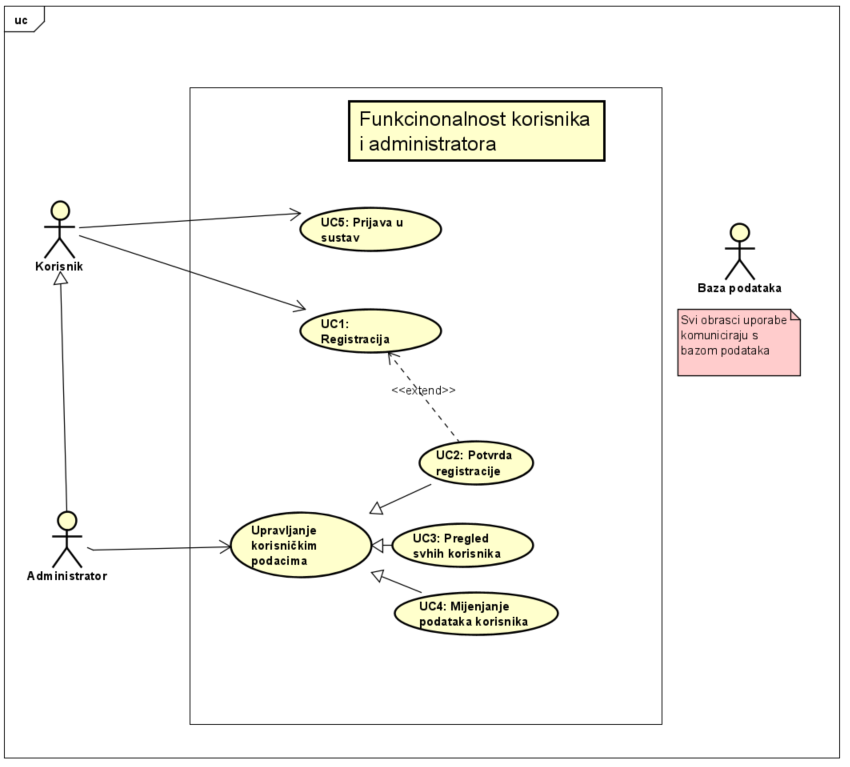
\includegraphics[scale=0.8]{dijagrami/Korisnik-admin-dijagram.PNG} 
						\centering
						\caption{Dijagram obrasca uporabe, funkcionalnost korisnika i administratora}
						\label{fig:promjene}
					\end{figure}	
					
					\begin{figure}[H]
						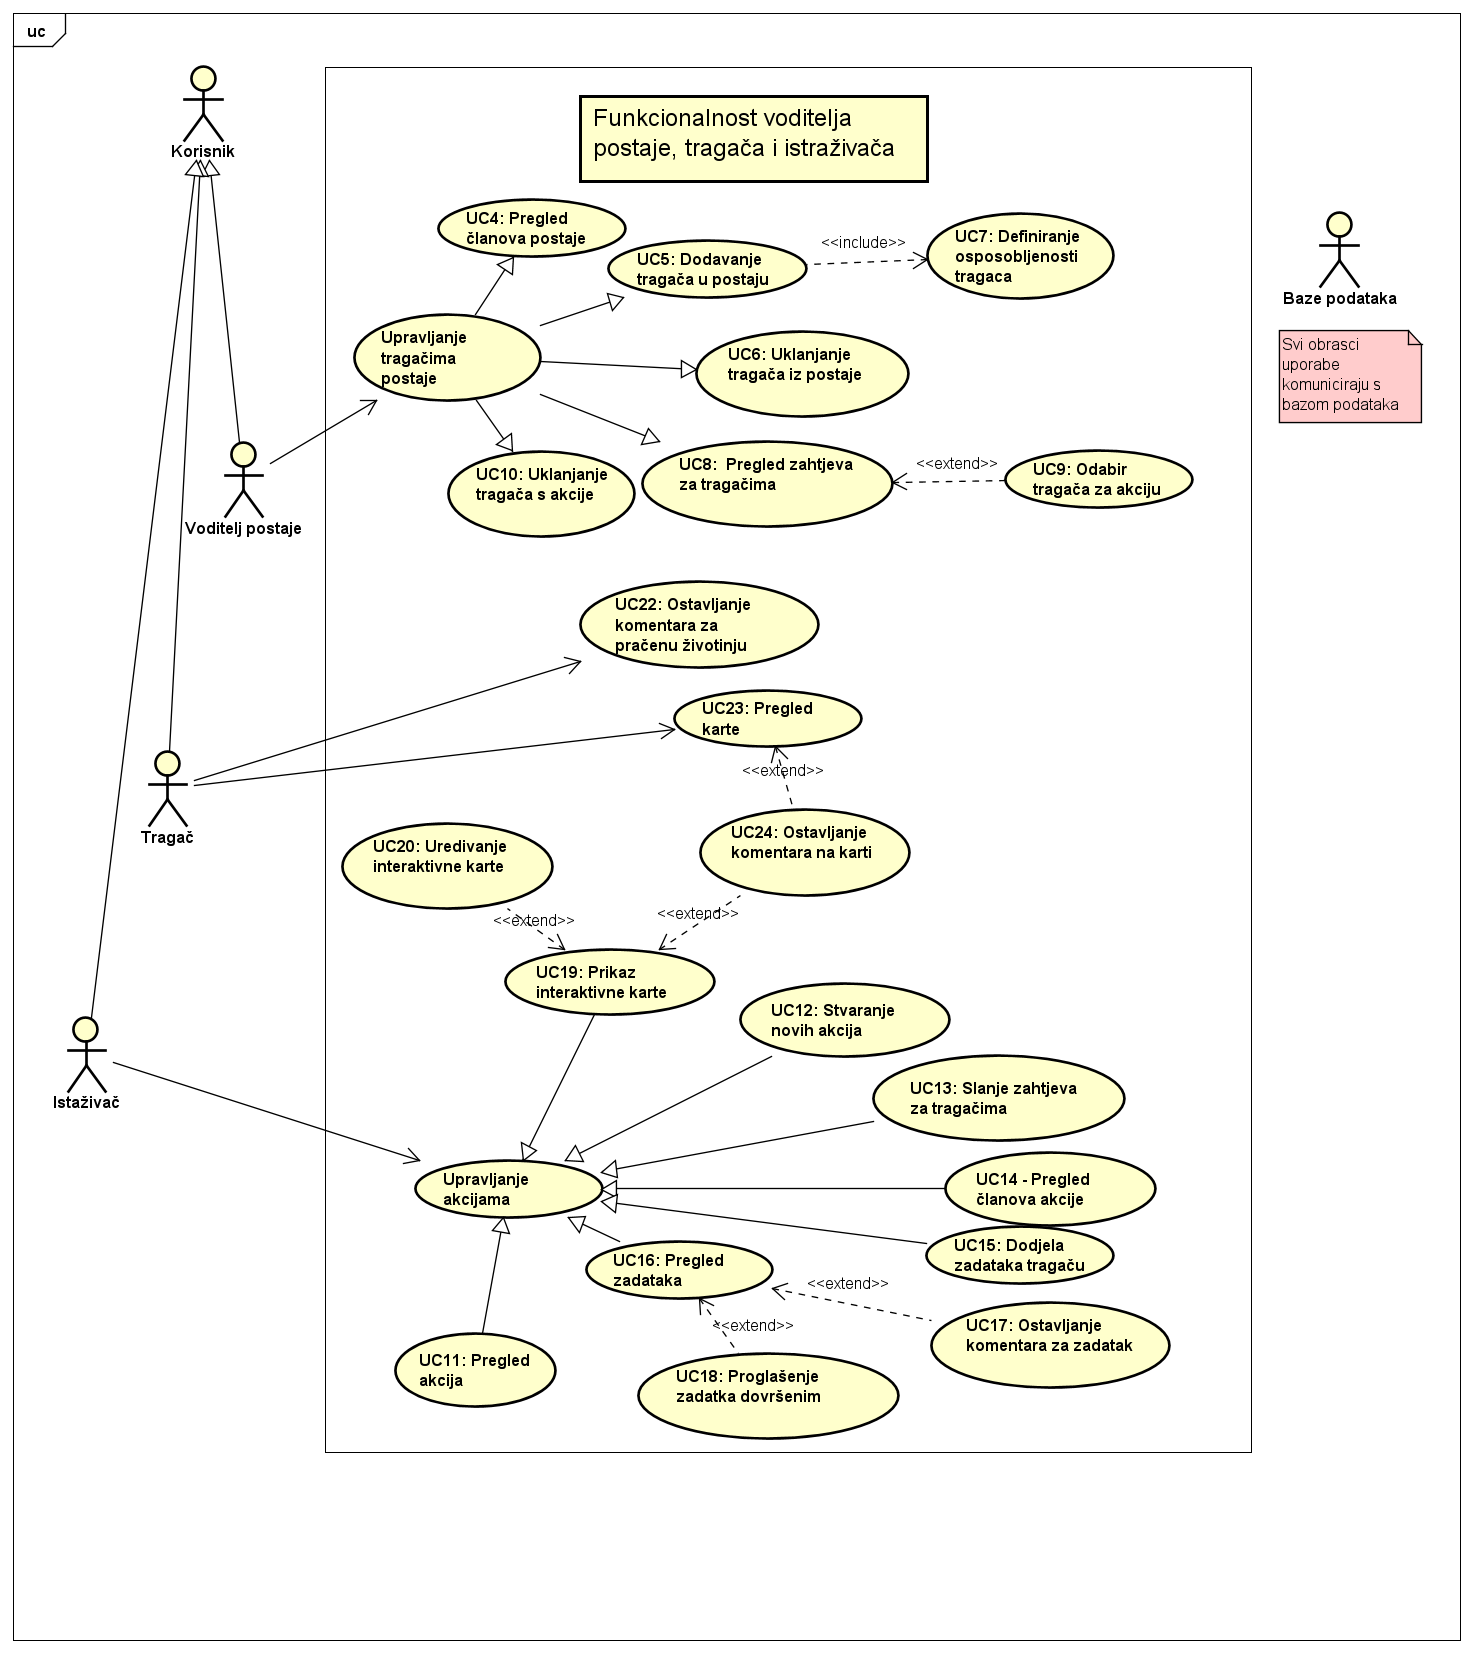
\includegraphics[scale=1]{dijagrami/voditelj-tragac-istrazivac-dijagram.PNG} 
						\centering
						\caption{Dijagram obrasca uporabe, voditelja postaje, tragača i istraživača}
						\label{fig:promjene}
					\end{figure}
					
			\eject				
				
			\subsection{Sekvencijski dijagrami}
			
				\subsubsection{Obrazac uporabe UC9 - Odabir tragača za akciju}
				Voditelj postaje šalje zahtjev za prikazom popisa pristiglih zahtjeva za alociranjem tragača za sudjelovanje u akciji. Poslužitelj dohvaća podatke o pristiglim zahtjevima i prikazuje ih. Voditelj odabire koji zahtjev želi detaljnije pregledati. Poslužitelj dohvaća pojedinosti o zahtjevu i prikazuje ih. Voditelj zatim šalje zahtjev za odabirom tragača koji će sudjelovati u akciji. Poslužitelj dohvaća tragače koji su raspoloživi. Raspoloživi tragači su oni koji u tom trenutku ne sudjeluju u niti jednoj akciji. U slučaju da takvih tragača ne postoji, poslužitelj ispisuje poruku "Nema raspoloživih tragača". U suprotnom, poslužitelj prikaže popis raspoloživih tragača.  Voditelj postaje zatim bira koje tragače želi dodati u akciju sve dok ne pošalje zahtjev za potvrdom odabira. Tada poslužitelj sprema odabir u bazu podataka.
				
				\eject
				
				\begin{figure}[H]
					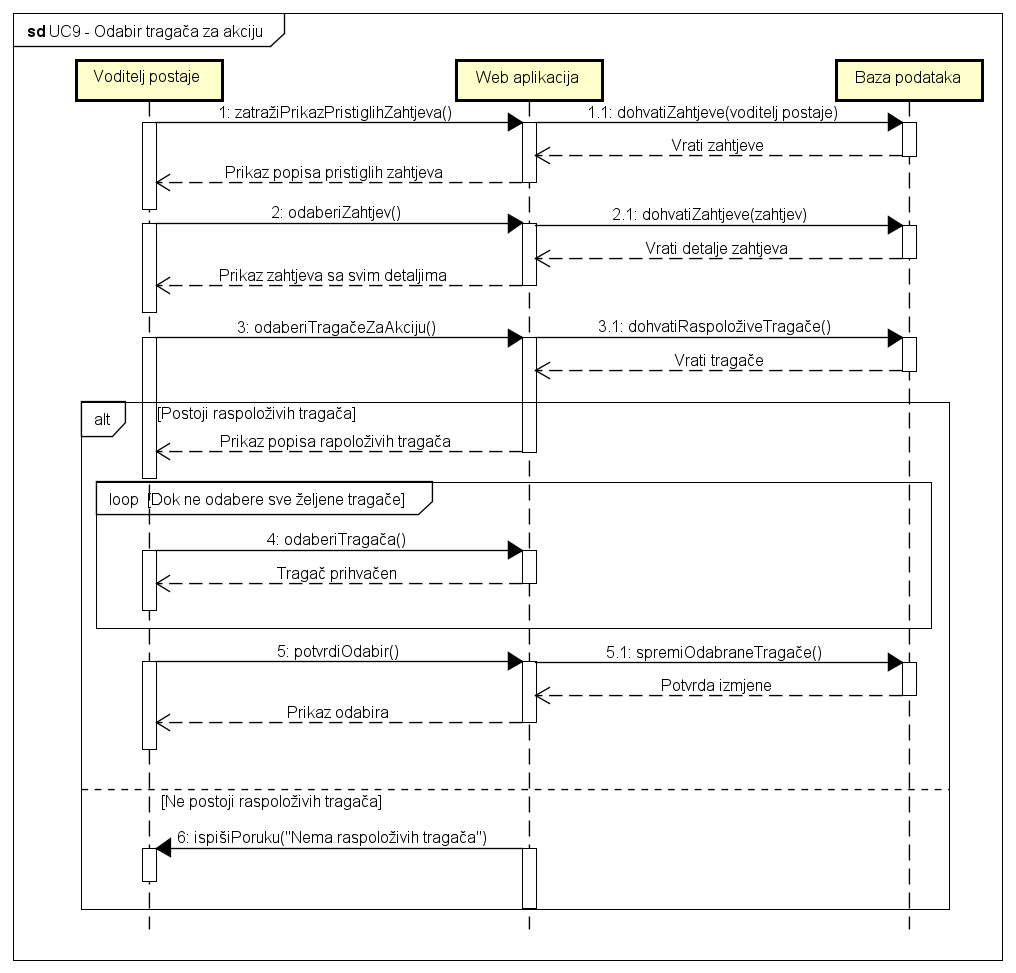
\includegraphics[scale=0.6]{dijagrami/UC9-Odabir tragača za akciju} 
					\centering
					\caption{Sekvencijski dijagram za UC9}
					\label{fig:promjene}
				\end{figure}
				
				\eject
				
				\subsubsection{Obrazac uporabe UC15 - Dodjela zadatka tragaču}
				Istraživač šalje zahtjev za prikazom akcija u kojima sudjeluje. Poslužitelj dohvaća podatke o istraživačevim akcijama i prikazuje ih. Istraživač odabire koju akciju želi detaljni pregledati. Poslužitelj dohvaća pojedinosti o akciji i prikazuje ih. Istraživač zatim šalje zahtjev za pregled tragača koji sudjeluju u akciji. Poslužitelj dohvaća tragače koji sudjeluju u akciji i prikazuje ih. Istraživač odabire tragača i poslužitelj bilježi taj odabir. Istraživač zatim šalje zahtjev o dodjeli zadatke odabranom tragaču. Poslužitelj dohvaća spremljenu kartu korištenu za ovu akciju i prikazuje ju zajedno s dijelom namijenjenim za odabir uređaja kojeg istraživač želi da se postavi(kamera ili uređaj za praćenje). Istraživač zatim na karti označava kojom rutom želi da se tragač kreće i do koje odredišne lokacije. Poslužitelj bilježi odabranu rutu. Istraživač onda bira između ponuđenih uređaja što poslužitelj također bilježi. Na kraju, istraživač potvrđuje dodjelu zadatka odabranom tragaču. Poslužitelj sprema u bazu podataka novi zadatak s svim navedenim specifikacijama i naznačuje tragača kojem je namijenjen. 
				
				\eject
				
				\begin{figure}[H]
					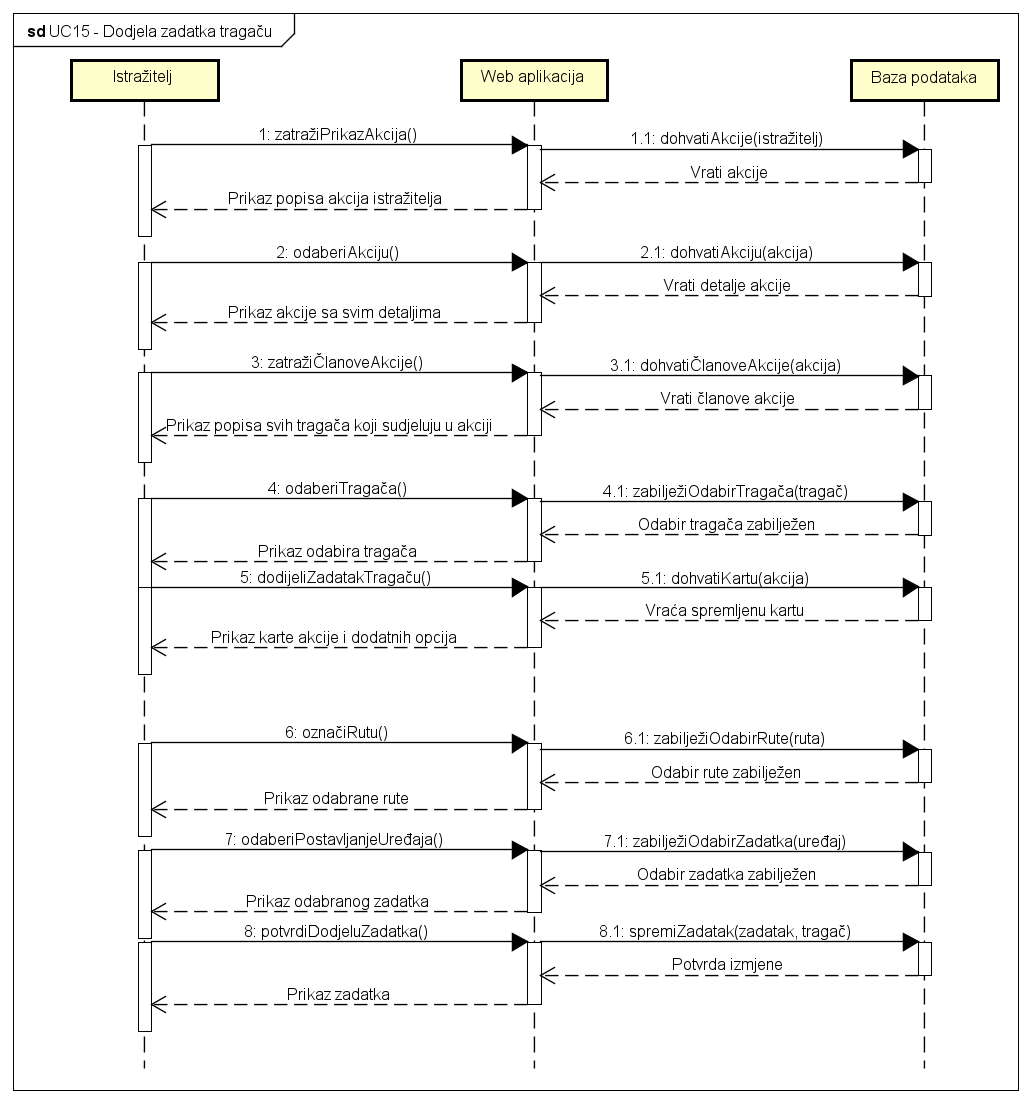
\includegraphics[scale=0.6]{dijagrami/UC15-Dodjela zadatka tragaču} 
					\centering
					\caption{Sekvencijski dijagram za UC15}
					\label{fig:promjene}
				\end{figure}
				
				\eject
				
				
				\subsubsection{Obrazac uporabe U20 - Uređivanje interaktivne karte}
				Istraživač šalje zahtjev za prikazom interaktivne karte. Poslužitelj dohvaća podatke o posljednjom spremljenom odabiru o prikazu informacija na karti i prikazuje ih. Istraživač zatim šalje zahtjev o uređivanju karte. Poslužitelj dohvaća podatke o svim mogućim informacijama koje mogu biti prikazane na karti i prikazuje ih istraživaču. Istraživač sada šalje zahtjev s odabirom koje informacije želi da budu prikazane. Poslužitelj provjerava je li odabrana opcija prikaza povijesnih pozicija svih praćenih životinja ili povijesnih pozicija svih tragača koji sudjeluju u akciji. Ako jest, onda poslužitelj prikazuje opcije filtriranja. U slučaju prikaza povijesnih pozicija svih praćenih životinja, podaci mogu biti filtrirani po vrsti ili pojedinačno po jedinki, dok prikaz povijesnih pozicija svih tragača koji sudjeluju u akciji može biti filtriran po tipu prijevoza ili pojedinačno po tragaču. Istraživač šalje zahtjev s odabirom kako želi da informacija bude filtrirana. Poslužitelj dohvaća informaciju s primijenjenim filtriranjem iz baze podataka, a u slučaju da je pri odabiru informacija bio odabran prikaz trenutnih pozicija praćenih životinja ili tragača, onda poslužitelj dohvaća tu informaciju bez ikakvog dodatnog filtriranja. Istraživač zatim šalje potvrdu za primjenu novog uređenja. Poslužitelj zatim sprema odabir u bazu podataka te prikazuje novonastalu kartu.
				\eject
				\begin{figure}[H]
					\includegraphics[scale=0.5]{dijagrami/UC20-Uređivanje interaktivne karte.PNG} 
					\centering
					\caption{Sekvencijski dijagram za UC20}
					\label{fig:promjene}
				\end{figure}
				
			\eject
		\section{Ostali zahtjevi}
		
			\begin{itemize}
				\item Web aplikaciju treba implementirati koristeći objektno-orijentirane jezike.
				\item Korisničko sučelje pri unosu i prikazu podataka treba podržavati hrvatski jezik uključujući dijakritičke znakove. 
				\item Potrebno je osigurati obranu sustava od pogrešnog korištenja korisničkog sučelja s dodatnim provjerama valjanosti.
				\item Sustav mora podržavati veći broj korisnika u stvarnom vremenu.
				\item Korisničko sučelje mora biti jednostavno i intuitivno za uporabu.
				\item Sustav je potrebno oblikovati na način koji pridonosi ponovnoj uporabi kao što je uvođenje kopči u program. 
				\item Programska potpora treba biti pripremljena za moguće promjene u budućnosti. 
				\item Sustav mora odgovoriti na zahtjev korisnika u roku od nekoliko sekundi. 
				\item Pristup bazi podataka mora biti dobro zaštićen. 
				\item Dohvat sadržaja iz baze podataka trebao bi biti brz i učinkovit. 
				\item Programski proizvod treba raditi na što većem broju različitih platformi što se omogućuje korištenjem programskih jezika neovisnih o platformi.
				\item Komunikacija između web klijenta i web poslužitelja odvija se preko HTTPS protokola. 
			\end{itemize}
		 
			 
			 
			 
	